\documentclass[a4paper,12pt]{article}

% ================================================== DATOS ==================================================

% Información de la materia
\newcommand{\codMateria}{TA135}
\newcommand{\nombreMateria}{Taller de}
\newcommand{\cuatrimestre}{1.\textsuperscript{er} Cuatrimestre}

% Información del TP
\newcommand{\TpTitulo}{Trabajo Práctico n.° 2}
\newcommand{\fecha}{\today}
\newcommand{\group}{Grupo 7}

% Información de alumnos
\newcommand{\nombreA}{Lautaro García Vitale}
\newcommand{\padronA}{110028}
\newcommand{\emailA}{lagarciav@fi.uba.ar}

\newcommand{\nombreB}{Santiago Manuel Cabrera}
\newcommand{\padronB}{110445}
\newcommand{\emailB}{smcabrera@fi.uba.ar}

% ================================================== PAQUETES =================================================

% Codificación y lenguaje
\usepackage[utf8]{inputenc}
\usepackage[ddmmyy]{datetime}
\usepackage[language=spanish]{lipsum}
\usepackage[spanish]{datetime2}
\usepackage[T1]{fontenc}
\usepackage[spanish,es-nodecimaldot]{babel}
\usepackage[a4paper,margin=2.5cm]{geometry}
\usepackage{amsmath,amssymb,amsthm,mathtools}
\usepackage{bm}
\usepackage{physics}
\usepackage{setspace}
\usepackage{hyperref}
\usepackage{enumitem}

% Márgenes y página
\usepackage{geometry}
\usepackage{fancyhdr}
\usepackage{emptypage}
\usepackage{parskip}

% Encabezado personalizado
\pagestyle{fancy}
\fancyhf{}
\rhead{\group}
\lhead{\TpTitulo}
\cfoot{\thepage}

% Tipografía matemática
\usepackage{mathtools}
\usepackage{amssymb}
\usepackage{amsfonts}
\usepackage{amsthm}
\usepackage{yhmath}
\usepackage{dsfont}
\usepackage{esdiff}
\usepackage{xfrac}
\usepackage{siunitx}
\sisetup{per-mode=reciprocal, separate-uncertainty=true}

% Gráficos y tablas
\usepackage{graphicx}
\usepackage{float}
\usepackage{booktabs}
\usepackage{caption}
\usepackage{subcaption}
\usepackage{multirow}
\usepackage{adjustbox}
\usepackage[spanish]{babel}
\addto\captionsspanish{
  \renewcommand{\tablename}{Tabla}
}

% TikZ y gráficos avanzados
\usepackage{pgfplots}
\pgfplotsset{compat=1.18}
\usepackage{tikz}

% Código fuente y resaltado
\usepackage{minted}
\usepackage{tcolorbox}
\definecolor{codebg}{rgb}{0.95,0.95,0.95}  % Color de fondo del código
\usemintedstyle{friendly}                  % Estilo del resaltado de sintaxis
\setminted{
    linenos=true,                          % Numeración de líneas
    bgcolor=codebg,                        % Color de fondo del código
    fontsize=\footnotesize,                % Tamaño de la fuente
    frame=lines,                           % Estilo del marco
    framesep=2mm,                          % Separación del marco
    baselinestretch=1.2,                   % Espaciado entre líneas
    breaklines=true,                       % Romper líneas largas automáticamente
    encoding=utf8,                         % Codificación del archivo
    tabsize=4,                             % Tamaño de la tabulación
}

% Misceláneo
\usepackage{anyfontsize}
\usepackage{xcolor}
\usepackage{url}
\usepackage{comment}
\usepackage{multicol}
\usepackage[numbers,square]{natbib}

% Estilo de bibliografía
\bibliographystyle{IEEEtran}


% ==============================================================================================================
% ==============================================================================================================


\begin{document}

% ================================================== CARÁTULA ==================================================

\pagenumbering{arabic} % Comienza la numeración

\vspace{-1 cm} % La primera hoja tiene que tener menos espaciado

\begin{center}
  \begin{minipage}{0.8 cm}
    
\includegraphics[width=\linewidth]{img/fiuba.png}
  \end{minipage}
  \begin{minipage}{\widthof{\large{\textsc{Universidad de Buenos Aires}}}}
    \centering
    \large{\textsc{Universidad de Buenos Aires}}\\
    \large{\textsc{Facultad de Ingeniería}}\\
    \small{Año 2026 -- \cuatrimestre}
  \end{minipage}
\end{center}
\vspace{10mm}
\begin{center}
  \huge{\underline{\textsc{\nombreMateria}}} \\
  \huge{\underline{\textsc{Automatización y Control}}} \\
  \vspace{7 pt}
  \Large{\TpTitulo \\}
  \vspace{3mm}
  \large{\group}
\end{center}

\newcommand{\anchopadron}{\widthof{000 000}}
\begin{center}
  \begin{tabular}{l l l}
    \nombreA & \parbox{\anchopadron}{\raggedleft \padronA} & \emailA \\
    \nombreB & \parbox{\anchopadron}{\raggedleft \padronB} & \emailB
  \end{tabular}
\end{center}
\vspace{8mm}

\begin{center}
\renewcommand{\arraystretch}{1.3}
\begin{tabular}{@{}r p{0.62\textwidth}@{}}
\textbf{Docentes:} & Dr. Ing. Claudio Pose -- Ing. Tomás González.
\end{tabular}
\end{center}

\vspace{2em}
\thispagestyle{empty}

\begin{abstract}
En este trabajo práctico se estudia el modelado, identificación y control digital de un sistema \textit{Ball and Beam}. A partir de mediciones experimentales se obtuvieron modelos para la dinámica servo-barra y barra-carrito, que luego se combinaron para representar la planta completa mediante una función de transferencia y una descripción en espacio de estados. Sobre este modelo se analizaron las principales limitaciones de diseño, incluyendo la frecuencia de muestreo, los márgenes de estabilidad y la saturación de la acción de control. Finalmente, se diseñaron e implementaron controladores P, PI y PD, comparando sus respuestas simuladas y medidas. Los resultados permiten evaluar el compromiso entre velocidad de respuesta, estabilidad, esfuerzo de control y sensibilidad al ruido en la implementación real del sistema.
\end{abstract}

\newpage

\tableofcontents

\newpage

\section{Introducción}

En el presente trabajo práctico se aborda el análisis y control digital de un sistema del tipo \textit{Ball and Beam}, una planta clásica en el área de control automático debido a su naturaleza inherentemente inestable y a la necesidad de diseñar estrategias de realimentación capaces de estabilizarla. El sistema consiste en una barra cuya inclinación es comandada mediante un servomotor, provocando el desplazamiento lineal de un carro sobre dicha barra a causa de la componente tangencial de la gravedad.

El objetivo principal del trabajo es desarrollar un modelo matemático de la planta linealizado alrededor del punto de equilibrio, definido cuando la barra se encuentra horizontal y el carro ubicado en el centro de la misma. A partir de este modelo se busca estudiar las limitaciones dinámicas del sistema y diseñar distintos controladores digitales capaces de estabilizar y regular la posición del carro.

Para ello, se analizarán diferentes estrategias de control, incluyendo controladores proporcional (P), proporcional-integral (PI) y proporcional-derivativo (PD), evaluando tanto su desempeño en simulación como su implementación práctica sobre una plataforma basada en Arduino. Asimismo, se estudiará la influencia de parámetros fundamentales del diseño, tales como el ancho de banda, el esfuerzo de control, la estabilidad y la frecuencia de muestreo del sistema.

Finalmente, se compararán las respuestas obtenidas experimentalmente con aquellas predichas por el modelo teórico, permitiendo analizar las diferencias entre el comportamiento ideal y el real de la planta, así como las limitaciones inherentes al modelado y a la implementación física del controlador.

\newpage

\section{Sistemas de referencia}

\label{sec:Sistemas de referencia}

Se tiene una barra de 40 cm de longitud en cuyo borde se encuentra un sensor ultrasónico que ocupa 1 cm de la misma. Sobre ella se monta un carrito rodante de 5,5 cm. La posición del carrito sobre la barra es la salida del sistema ($y = x$), mientras que el ángulo comandado al servomotor es la acción de control ($u = \theta_s$).

En la Figura \ref{fig:planta} se observan los sistemas de referencia adoptados. Con la planta orientada de forma tal que el servomotor quede hacia adelante, la posición del carrito se toma positiva hacia la izquierda y su origen en el centro de la barra. Se modela al carrito como una masa puntual, por lo que su posición en verdad será la posición de su centro geométrico. Asimismo, se consideran positivos los ángulos antihorarios respecto de las horizontales.

\begin{figure}[H]
    \centering
    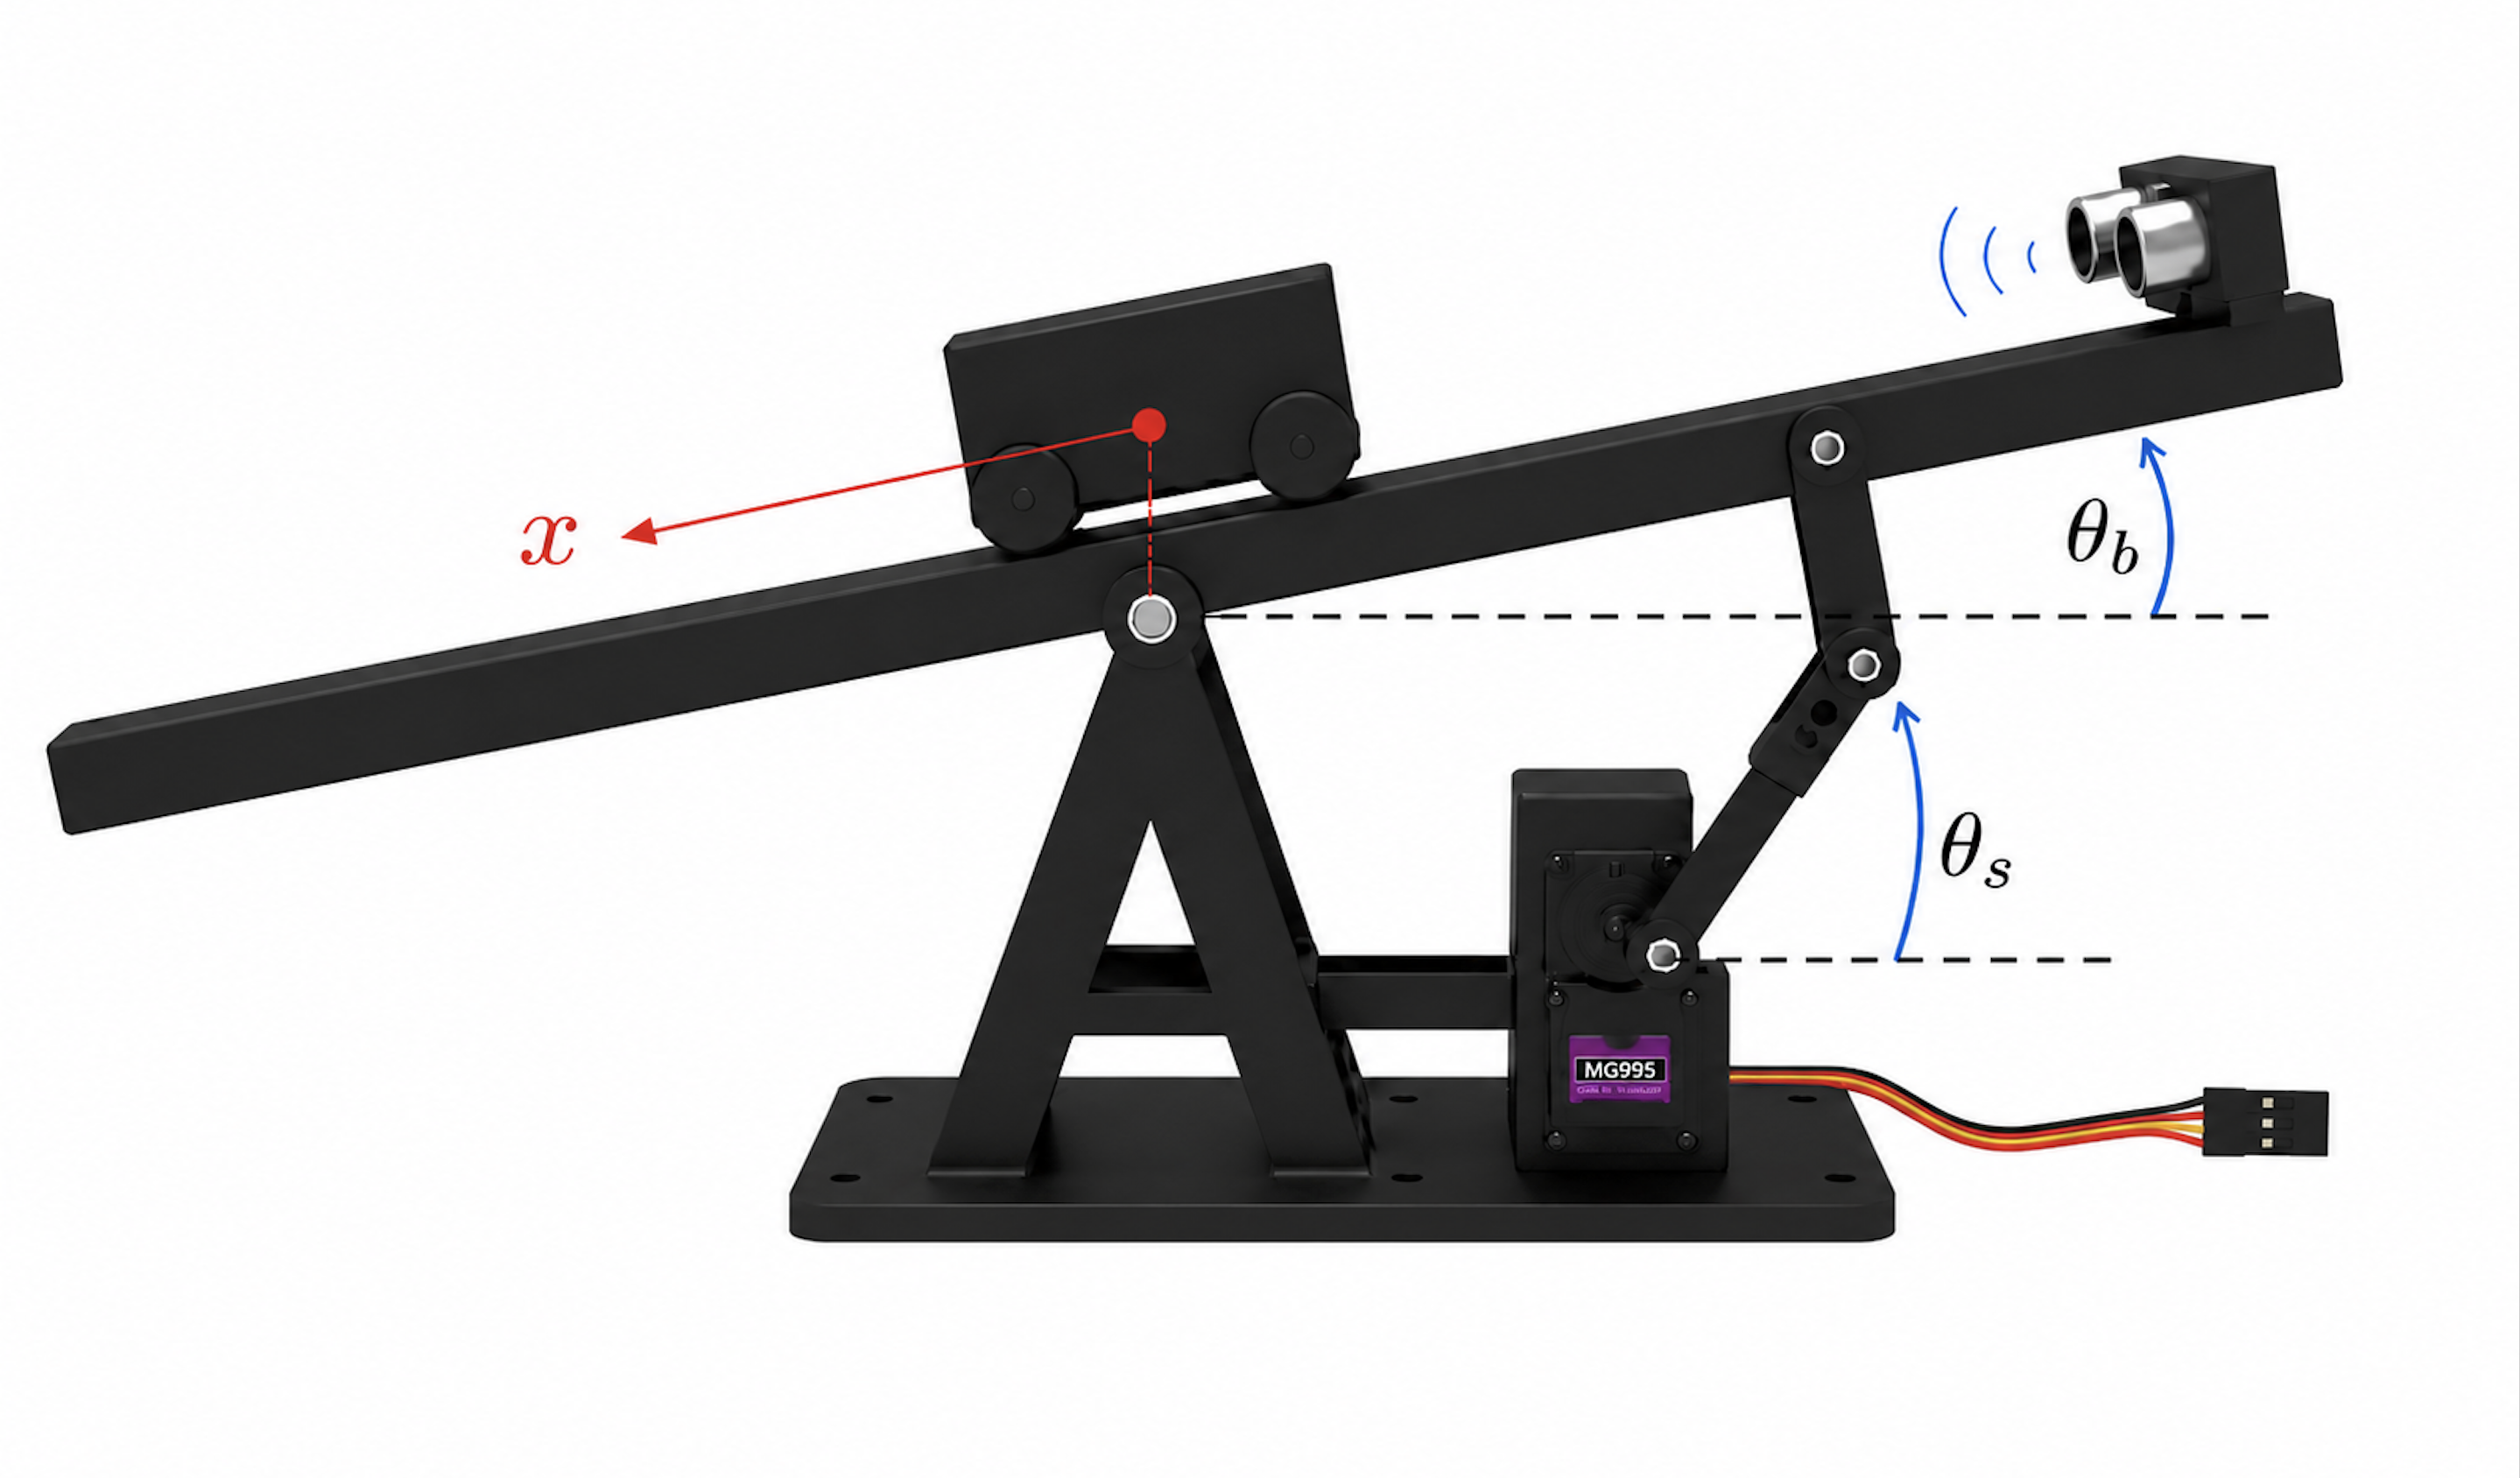
\includegraphics[width=1\textwidth]{img/planta.png}
    \caption{Esquema de la planta y sus sistemas de referencia.}
    \label{fig:planta}
    
\end{figure}

Nótese que la posición del carrito es una traducción de los datos brindados por el sensor ultrasónico, cuya zona muerta es de 2 cm, es decir, siempre que la pared derecha del carrito se encuentre a 2 cm o menos del sensor, el mismo arrojará una medición de 2 cm sin distinción.

De este modo, la posición del carrito verificará $x \in [-14,25\,\text{cm}; ~ 17,25\,\text{cm}]$. Si el carrito llegase a caerse de la barra o se agotara el tiempo de medición, la posición se forzará al origen del sistema de referencia.

Experimentalmente se observó que el ángulo de la barra verifica $\theta_b \in [-16\text{°}; ~ 20\text{°}]$. Teniendo en cuenta la ganancia en continua de la transferencia servo-barra se determinó que el ángulo del servo verifica $\theta_s \in [-46,84\text{°}; ~ 58,55\text{°}]$, dado que se tiene un sobrepico de prácticamente $0\,$\% en la transferencia servo-barra.

\section{Modelado e identificación}

En la siguiente sección se detallan los modelos obtenidos de las distintas transferencias en la planta. 

\subsection{Transferencia servo-barra}

Se inicia suponiendo una transferencia de segundo orden del siguiente estilo:

\[
H(s) = \frac{\Theta_b (s)}{\Theta_s (s)} = \frac{k_1}{(s - p_1)(s - p_2)}\,, 
\]

donde $\Theta_b(s)$ y $\Theta_s(s)$ son la transformada de Laplace de $\theta_b(t)$ y $\theta_s(t)$, respectivamente.

De este modo, se busca una transferencia discreta

\[
H_d (s) = \frac{\Theta_b (z)}{\Theta_s (z)} = \frac{b}{z^2 + a_1 z + a_2}\,,  
\]

donde $a_1$, $a_2$ y $b$ son los parámetros a ajustar, y $\Theta_b(z)$ y $\Theta_s(z)$ son la transformada Z de $\theta_b(t)$ y $\theta_s(t)$, respectivamente. Antitransformando se obtiene la ecuación en diferencias

\[
\theta_b[n] + a_1\,\theta_b[n-1] + a_2\,\theta_b[n-2] = b\,\theta_s[n-2]\,
\]

a coeficientes constantes ajustable mediante mínimos cuadrados.

El proceso de identificación consistió en la medición del ángulo de la barra utilizando la IMU, comandada por una señal cuadrada de $\pm 45$° como acción de control y a un período de muestreo $T_s = 50\,$Hz. 

Para obtener los resultados de la planta continua basta con aplicar el logaritmo y dividir por el período de muestreo a los valores discretos hallados. 

\[
\begin{cases}
k_1 = 11,4345 \\
p_1 = -4,8680 + 3,0753j \\
p_2 = -4,8680 - 3,0753j
\end{cases}
\]

En la Figura \ref{fig:comparacion servo-barra} se observa la respuesta a un tren de escalones de $\pm45$° a lazo abierto tanto del modelo estimado como de la transferencia real medida. El porcentaje de similitud resultó del $93,3\,$\%.

\begin{figure}[H]
  \centering
  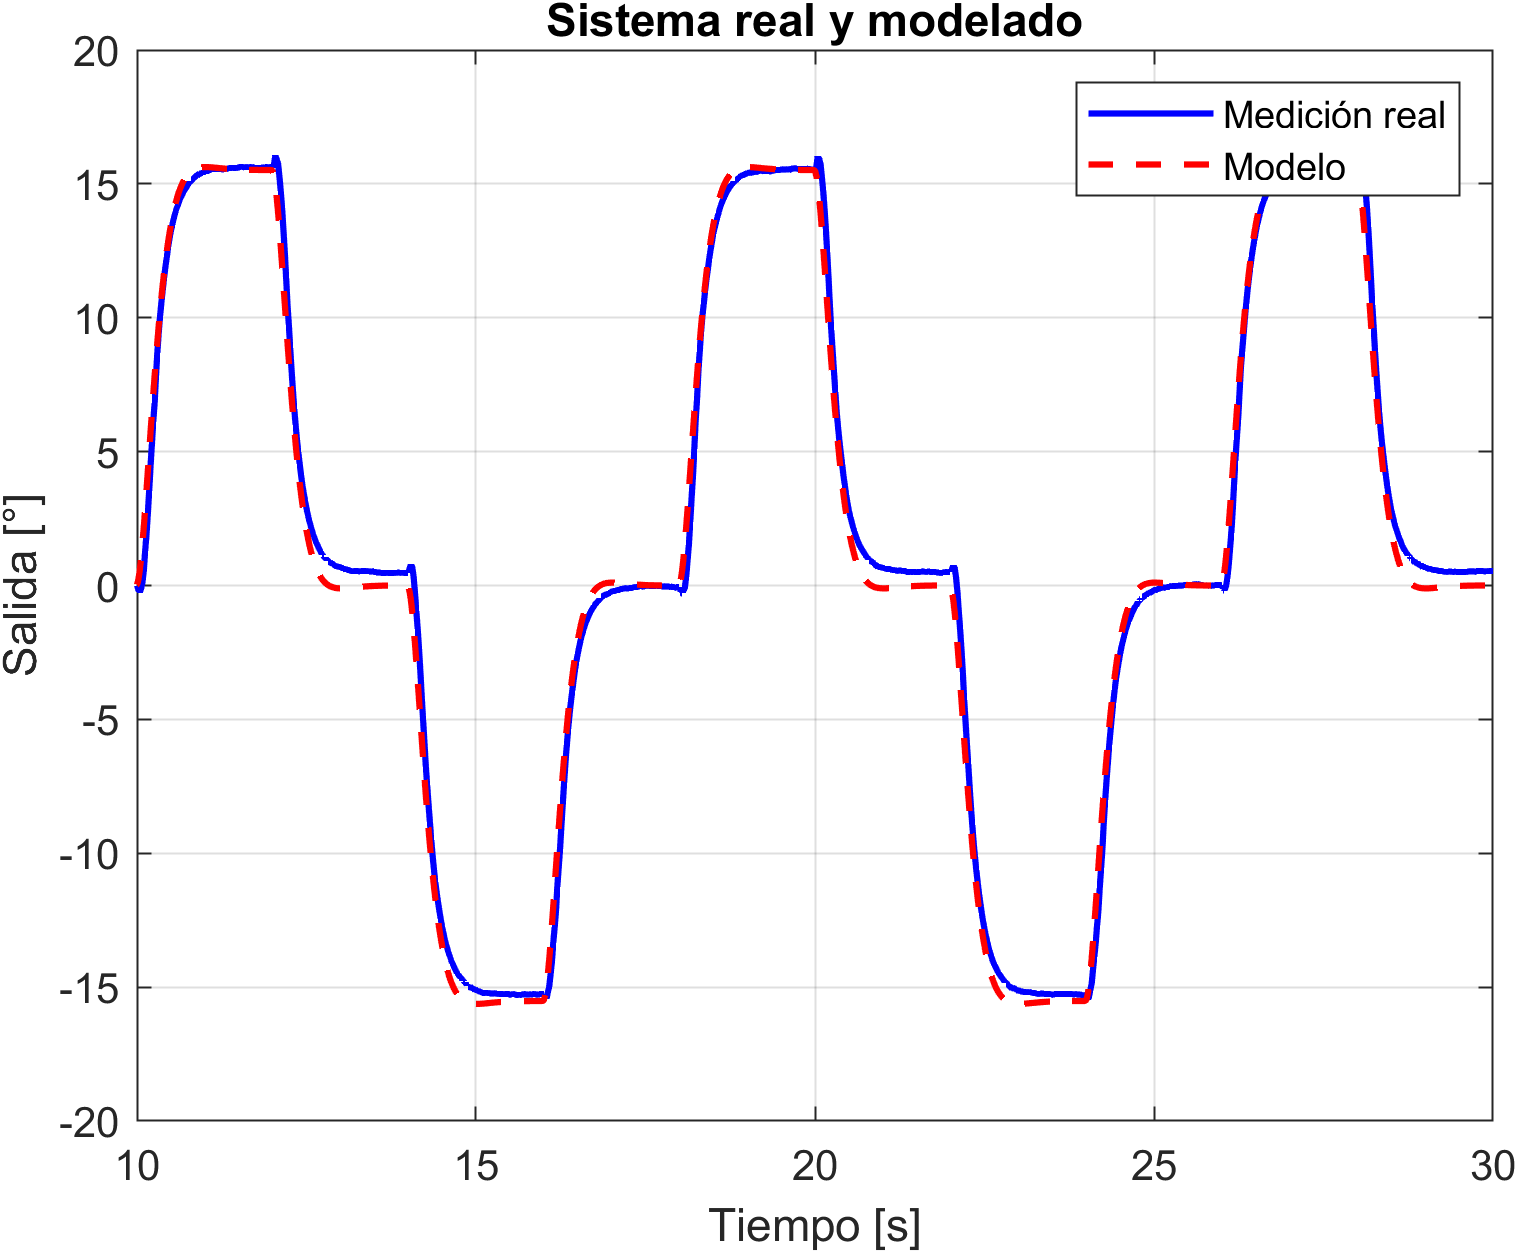
\includegraphics[width=0.8\textwidth]{img/Comparacion salidas(servo-barra).png}
  \caption{Comparación del modelo estimado con los datos medidos.}
  \label{fig:comparacion servo-barra}
\end{figure}

\subsection{Transferencia barra-carrito}

Para el cálculo de la dinámica de esta planta se idealizó al carrito como una masa puntual de masa $m = 33\,$g, considerando el peso del mismo a una aceleración de la gravedad $g = 9,8\,\mathrm{\sfrac{m}{s^2}}$, la normal que ejerce la barra sobre él y una fuerza viscosa con coeficiente de amortiguamiento viscoso $b$. Del diagrama de cuerpo libre y utilizando la Segunda Ley de Newton se obtiene la relación

\[
m \ddot{x} = m g \sen(\theta_b) - b \dot{x},
\]

donde se puede aproximar para ángulos pequeños $\sen(\theta_b) \approx \theta_b$. Transformando y despejando se obtiene

\[
\frac{X(s)}{\Theta_b(s)} = \frac{g}{s \left(s + \frac{b}{m}\right)}\,,
\]

siendo $X(s)$ la transformada de Laplace de $x(t)$.

Aquí, se tiene un polo en el origen y otro en $-\sfrac{b}{m}$.

Como se desea obtener una transferencia en $\sfrac{\mathrm{cm}}{\text{°}}$, se multiplica por un factor de conversión $f = 100\, \sfrac{\text{cm}}{\text{m}} \cdot \frac{\pi}{180\text{°}}$:

\[
\frac{X(s)}{\Theta_b(s)} = \frac{fg}{s \left(s + \frac{b}{m}\right)}\,.  
\]

De este modo, se busca una transferencia discreta

\[
\frac{X(z)}{\Theta_b(z)} = \frac{c}{(z-1)(z+a)}\,,  
\]

donde $a$ es el parámetro a ajustar, $c$ una ganancia determinada y $X(z)$ es la transformada Z de $x(t)$. Así, obtener la siguiente ecuación en diferencias

\[
x[n] = (1 - a)\,x[n-1] + a\,x[n-2] + c \theta_b[n-2]\,,
\]

donde hay tres parámetros a estimar: $\alpha_1 = 1 - a$, $\alpha_2 = a$ y $\alpha_3 = c$; y una restriccion: $\alpha_1 = 1 - \alpha_2$,  por lo que se utiliza mínimos cuadrados restringidos para ajustarlos.

El proceso de identificación consistió en la medición de la posición del carrito utilizando el sensor ultrasónico, comandado por un escalón de 20° como acción de control. Todos los datos a partir de la caída del carro se descartaron.

De esta manera, tras hacer varias mediciones y promediarlas, se obtuvo un coeficiente de amortiguamiento viscoso $b = 1,4505\,\sfrac{\text{kg}}{\text{s}}$, lo que ubica al polo en -43,9545.

Sin embargo, estos resultados no reflejaban con fidelidad el comportamiento real de la planta.

Experimentalmente se encontró que la dinámica de la planta se corresponde con un polo en $p_3 = -10$ y una ganancia 2,1 veces mayor a la modelada físicamente, $k_2 = 2,1 \cdot fg$. Estos valores fueron ajustados hasta reducir el error cuadrático medio entre la respuesta estimada y los datos medidos. Por tanto,

\[
G(s) = \frac{X(s)}{\Theta_b(s)} = \frac{k_2}{s(s-p_3)}\,.  
\]

En la Figura \ref{fig:comparacion barra-carro} se observa la respuesta al escalón a lazo abierto tanto del modelo estimado como de la transferencia real medida. El porcentaje de similitud resultó del $91,219\,$\%.

\begin{figure}[H]
  \centering
  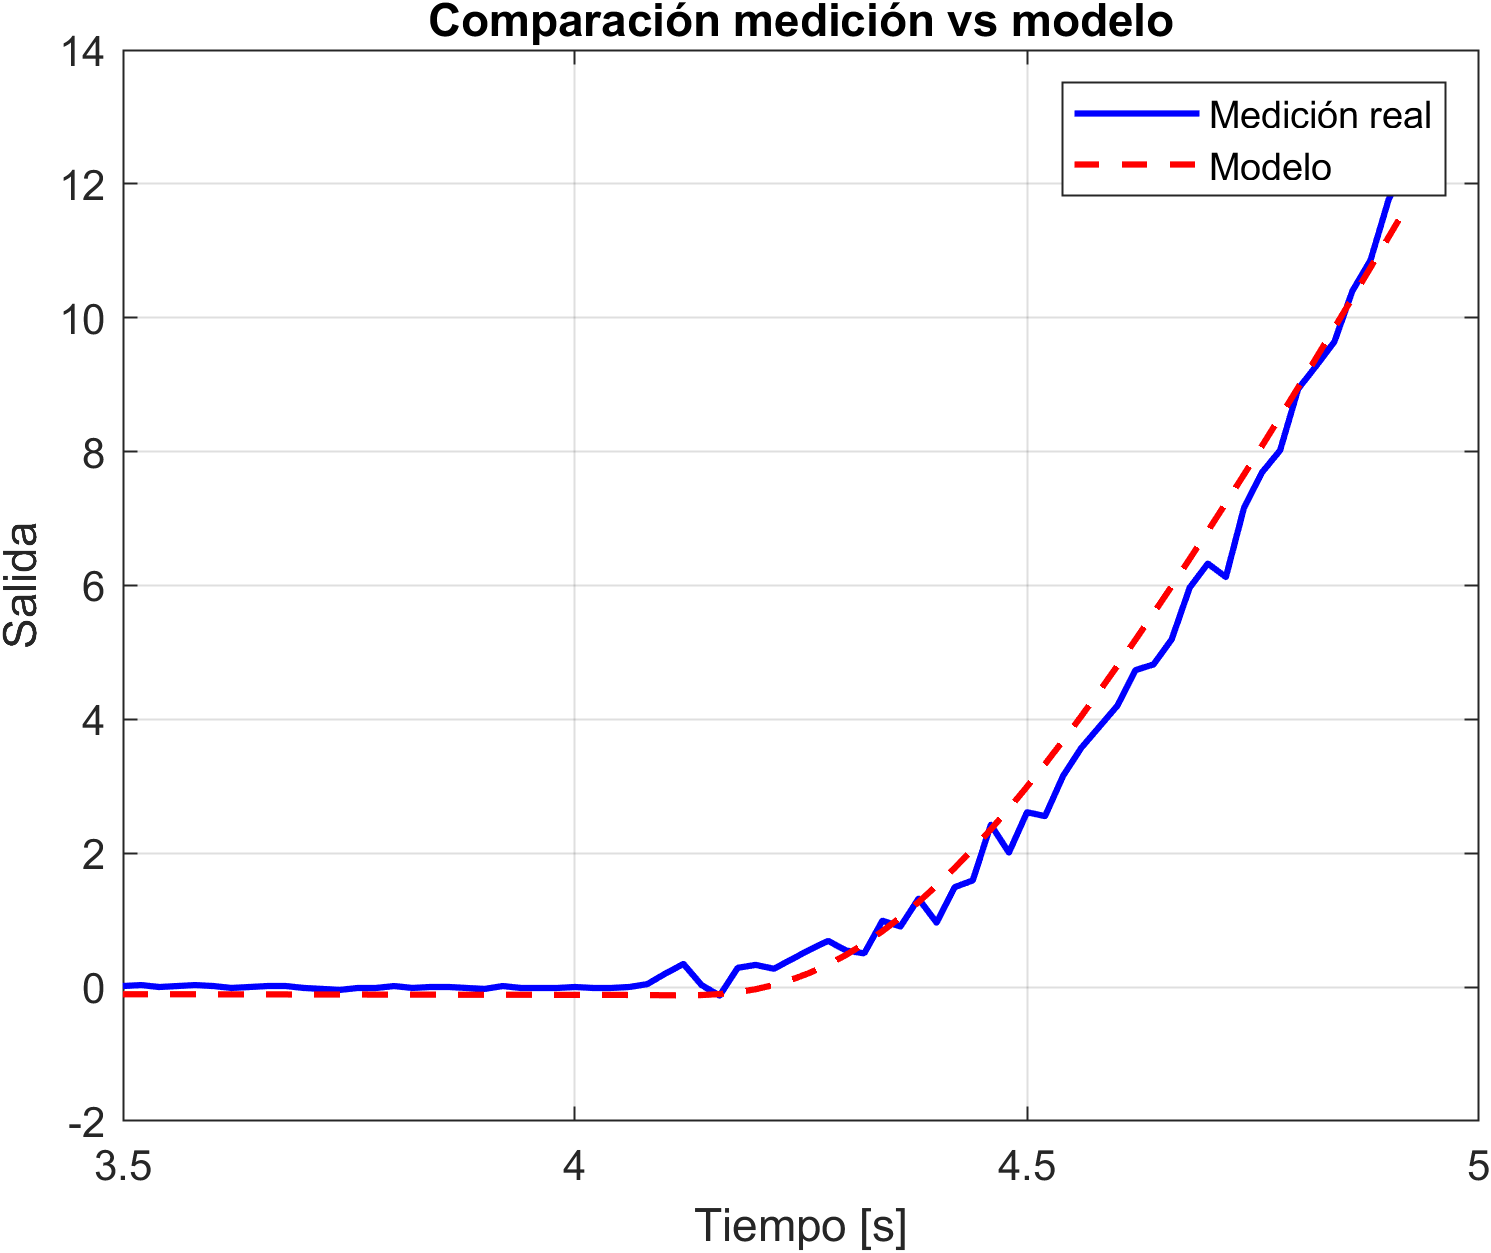
\includegraphics[width=0.8\textwidth]{img/Comparacion_modelado-real.png}
  \caption{Comparación del modelo estimado con los datos medidos.}
  \label{fig:comparacion barra-carro}
\end{figure}

\subsection{Planta final}

Sean $k = k_1k_2 = 410,7144$ y $P(s) = H(s)G(s)$.

Finalmente, la planta completa está dada por la siguiente función de transferencia.

\begin{align*}
P(s) = \frac{X(s)}{\Theta_s(s)} &= \frac{k}{s(s-p_1)(s-p_2)(s-p_3)} \\ 
     &= \frac{410,7144}{s(s + 4,8680 - 3,0753j)(s + 4,8680 + 3,0753j)(s + 10)} \\
     &= \frac{410,7144}{s^4 + 19,736 s^3 + 130,515 s^2 + 331,549 s}
\end{align*}


\section{Descripción en espacio de estados}

Para hallar un sistema en variables de estado de la planta total se hallaron las ecuaciones diferenciales que definen a cada subsistema a partir de las transferencias identificadas. Se definen las siguientes variables de estado.

\[
\begin{cases}
x_1 = \theta_b : \text{ángulo de la barra} \\
x_2 = \dot{\theta_b}: \text{velocidad angular de la barra} \\
x_3 = x : \text{posición del carro} \\
x_4 = \dot{x}_3: \text{velocidad del carro}
\end{cases}
\]

Además, debe tenerse en cuenta que la entrada del sistema es el ángulo comandado al servo ($u = \theta_s$) y la salida del mismo es la posición del carro ($y = x_3$). Por último, debe considerarse que la salida del primer sistema es la entrada del segundo.

Hechas estas aclaraciones, se pueden obtener las ecuaciones diferenciales a partir de las transferencias halladas. Para el primer sistema se tiene la relación $\dot{x}_1 = x_2$.

\begin{equation*}
  H(s) = \frac{\Theta_b(s)}{\Theta_s(s)} = \frac{X_1(s)}{U(s)} = \frac{k_1}{s^2 - (p_1 + p_2)s + p_1p_2}
\end{equation*}

\begin{equation*}
  \ddot{x}_1 - (p_1 + p_2) \dot{x}_1 + p_1p_2 x_1 = k_1 u
\end{equation*}

\begin{equation*}
  \dot{x}_2 = - p_1p_2 x_1 + (p_1 + p_2) x_2 + k_1 u
\end{equation*}

Se tiene entonces para el primer sistema

\[
\begin{cases}
\dot{x}_1 = x_2 \\
\dot{x}_2 = - p_1p_2 x_1 + (p_1 + p_2) x_2 + k_1 u
\end{cases}.
\]

De forma análoga, para el segundo sistema se tiene lo siguiente.

\begin{equation*}
  G(s) = \frac{X(s)}{\Theta_b(s)} = \frac{X_3(s)}{X_1(s)} = \frac{k_2}{s (s - p_3)}
\end{equation*}

\begin{equation*}
  \ddot{x}_3 - p_3 \dot{x}_3= k _2 x_1 
\end{equation*}

\begin{equation*}
  \dot{x}_4 = p_3 x_4 + k_2 x_1
\end{equation*}

Combinando estos resultados se obtiene:

\[
\begin{cases}
\dot{x}_1 = x_2 \\
\dot{x}_2 = - p_1p_2 x_1 + (p_1 + p_2) x_2 + k_1 u \\
\dot{x}_3 = x_4 \\
\dot{x}_4 = k_2 x_1 + p_3 x_4
\end{cases},
\]

de lo cual se pueden obtener las matrices que representan al sistema en espacio de estados. 

\[
\begin{minipage}{0.45\textwidth}
\[
A =
\begin{bmatrix}
0 & 1 & 0 & 0 \\
-33,1549 & -9,7360 & 0 & 0 \\
0 & 0 & 0 & 1 \\
35,9445 & 0 & 0 & -10
\end{bmatrix}
\]
\end{minipage}
\hfill
\begin{minipage}{0.25\textwidth}
\[
B =
\begin{bmatrix}
0 \\
11,4345 \\
0 \\
0
\end{bmatrix}
\]
\end{minipage}
\]

\[
\begin{minipage}{0.35\textwidth}
\[
C =
\begin{bmatrix}
0 & 0 & 1 & 0
\end{bmatrix}
\]
\end{minipage}
\hfill
\begin{minipage}{0.25\textwidth}
\[
D =
\begin{bmatrix}
0
\end{bmatrix}
\]
\end{minipage}
\]


\section{Limitaciones de diseño}

\begin{figure}[H]
  \centering
  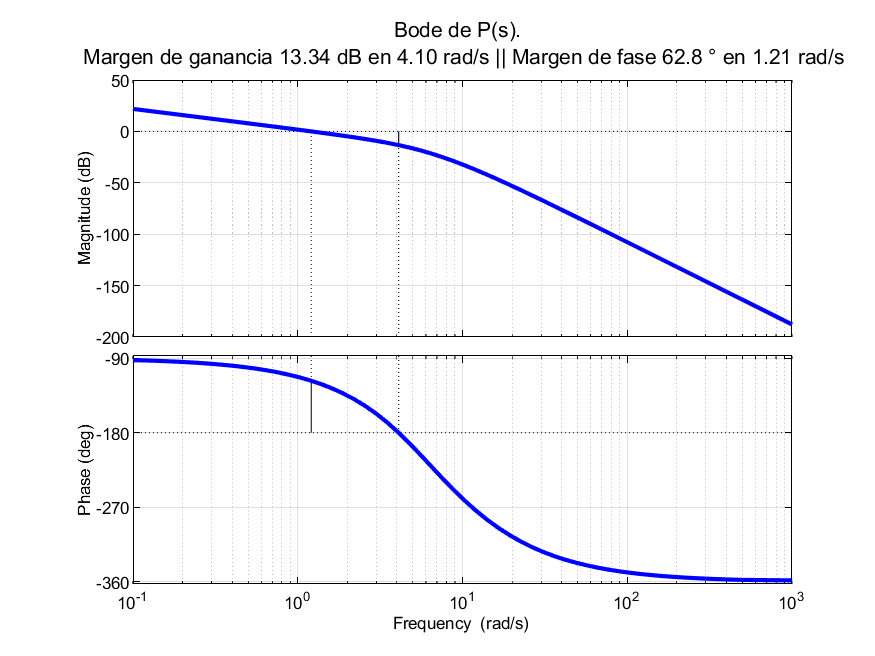
\includegraphics[width=0.8\textwidth]{img/Bode de la planta.png}
  \caption{Diagrama de Bode de la planta}
  \label{fig:bode de la planta}
  
\end{figure}

La principal limitación de diseño está dada por la frecuencia de control, la cual es de \SI{50}{\Hz}. De esta forma, todos los polos y ceros que se agreguen en el controlador deben estar por debajo de la frecuencia de Nyquist $f_N = \SI{25}{\Hz}$. De lo contrario, introducirían dinámicas muy rápidas que no podrían ser percibidas por los sensores. 

Por otro lado, ya que la planta no tiene polos ni ceros en el semiplano derecho, no hay restricciones para ubicar la frecuencia de cruce por cero $\omega_{gc}$ además de la ya mencionada. 

Como tercera limitación importante se destaca el margen de ganancia, $G_m = 13,34 \SI{}{\dB}$ (o, lo que es equivalente $G_m = 4,64$). De esta forma, se tiene un rango de valores posibles para $k_p$, $0 < k_p < 4,64$. 

La última limitación importante la dan los límites de la acción de control detallados en la Sección \ref{sec:Sistemas de referencia}, $ -46,84 \text{°} < u < 58,55 \text{°}$. Se deben diseñar controladores que no saturen la acción de control. 

Diseñar un controlador con mayor ancho de banda permite ubicar la frecuencia $\omega_{gc}$ en valores mayores, lo que aumenta el ancho de banda de la transferencia de lazo cerrado $T(s)$. Esto permite un mejor seguimiento de referencias de alta frecuencia, pero a su vez requiere de una acción de control mayor y tiende a hacer inestable al sistema.


\section{Diseño de controladores}

Para controlar la planta se utilizará un controlador PID de la forma

\begin{equation}
  C(s) = k_p + k_i \frac{1}{s} + k_d s\,.
  \label{eq:PID continuo}
\end{equation}

Para implementarlo en un microcontrolador, se discretizó $C(s)$ utilizando el método bilineal. Esta discretización da la siguiente fórmula para calcular la acción de control:

\begin{equation}
  u_k = k_p e_k + k_i I_k + k_d D_k\,,
  \label{eq:PID discreto}
\end{equation}

donde $u_k$ es el ángulo comandado al servomotor y 

\begin{equation}
  I_k = \frac{T_s}{2}(e_k + e_{k-1}) + I_{k-1}\,;
  \label{eq:integral discreta}
\end{equation}


\begin{equation}
  D_k = \frac{2}{T_s}(e_k - e_{k-1}) - D_{k-1}\,.
  \label{eq:derivada discreta}
\end{equation}

\subsection{Proporcional (P)}

Para el diseño de este controlador se eligió $k_p = 3,5$ resultante de una relación de compromiso entre el margen de fase y la rapidez del controlador. En la Figura \ref{fig:bode_p} se puede observar el diagrama de Bode a lazo abierto con sus respectivos márgenes de fase y ganancia.

\begin{figure}[H]
  \centering
  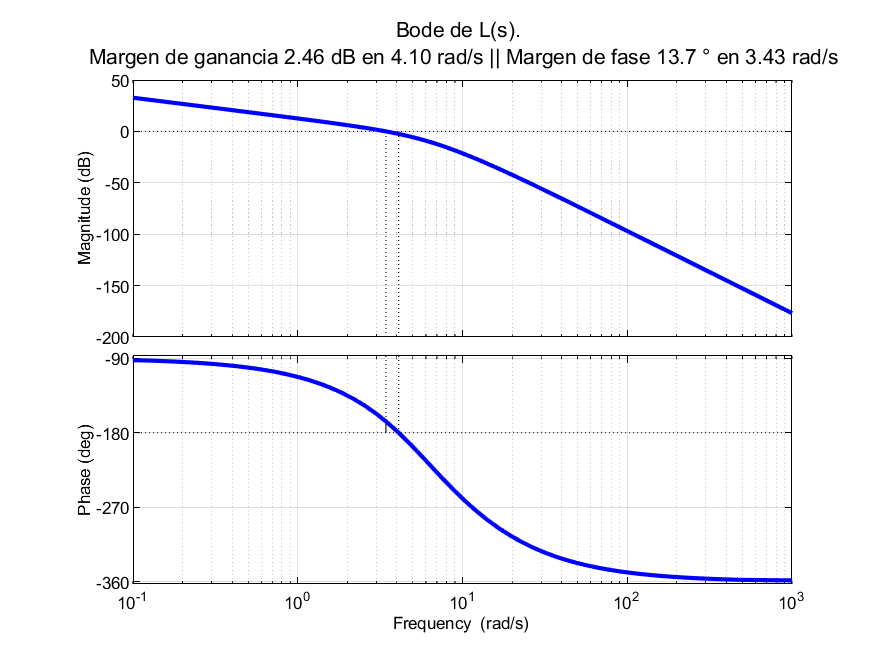
\includegraphics[width=0.75\textwidth]{img/P/Proporcional-Bode de L.png}
  \caption{Diagrama de Bode de $L(s)$.}
  \label{fig:bode_p}
\end{figure}

En las Figuras \ref{fig:impulso_p} y \ref{fig:escalon_p} se observan las respuestas al impulso y al escalón a lazo abierto medidas y simuladas, respectivamente.

\begin{figure}[H]
  \centering
  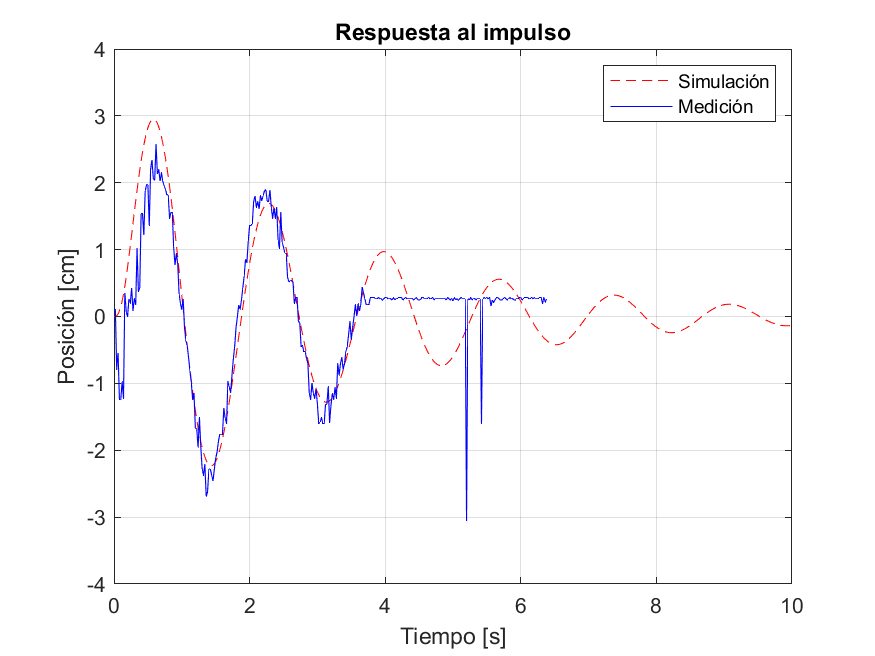
\includegraphics[width=0.75\textwidth]{img/P/proporcional-respuesta al impulso.png}
  \caption{Respuesta al impulso de $T(s)$.}
  \label{fig:impulso_p}
\end{figure}

\begin{figure}[H]
  \centering
  
\includegraphics[width=0.75\textwidth]{img/P/proporcional-respuesta al escalón.png}
  \caption{Respuesta al escalón de $T(s)$.}
  \label{fig:escalon_p}
\end{figure}

La estabilización cerca de la referencia, mas no en ella se debe al rozamiento intrínseco de la barra y ruedas del carrito. Esto se corregirá con una componente integradora en el controlador.

\subsection{Proporcional-Integrador (PI)}

De manera análoga al diseño anterior, se optó por los valores $k_p = 2$ y $k_i = 0,9$. En la Figura \ref{fig:bode_pi} se puede observar el diagrama de Bode a lazo abierto con sus respectivos márgenes de fase y ganancia.

\begin{figure}[H]
  \centering
  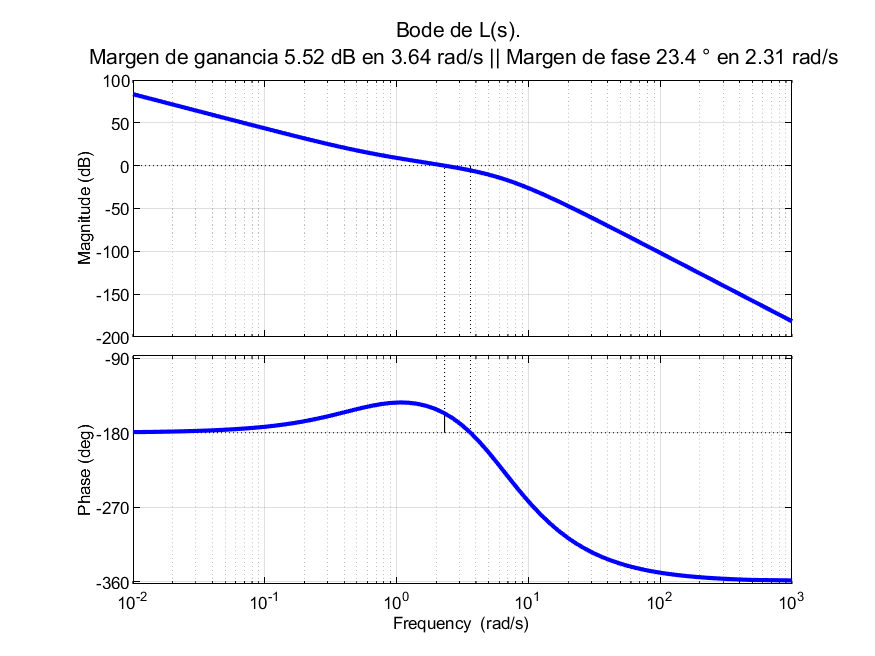
\includegraphics[width=0.75\textwidth]{img/PI/PI-Bode de L.png}
  \caption{Diagrama de Bode de $L(s)$.}
  \label{fig:bode_pi}
\end{figure}

En las Figuras \ref{fig:impulso_pi} y \ref{fig:escalon_pi} se observan las respuestas al impulso y al escalón a lazo cerrado medidas y simuladas, respectivamente. En las Figuras \ref{fig:control_impulso_pi} y \ref{fig:control_escalon_pi} se muestran sus respectivas acciones de control.

La acción integral del controlador PI acumula el error entre la referencia y la salida, aumentando o disminuyendo la acción de control mientras dicho error persista. De esta forma, aunque exista una desviación sostenida, el término integral continúa actuando hasta reducirla y hacer que la respuesta se acerque a la referencia. Esto se observa en los gráficos de acción de control: ante el impulso aparece una corrección rápida que luego disminuye a medida que el error se atenúa, mientras que ante el escalón la acción de control se ajusta de forma más sostenida hasta alcanzar el valor necesario para compensar el error en régimen permanente.

\begin{figure}[H]
  \centering
  \begin{minipage}{0.5\textwidth}
    \centering
    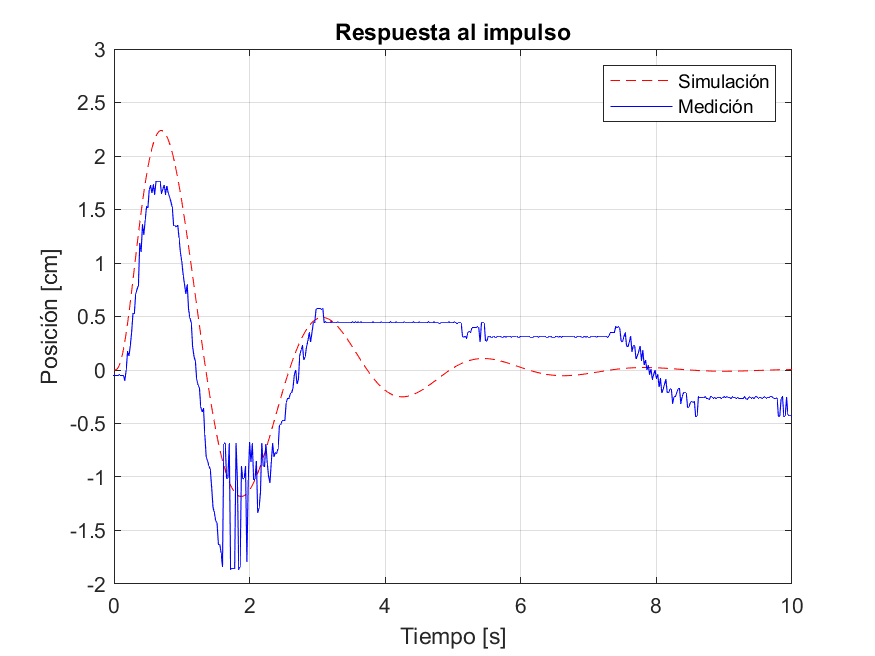
\includegraphics[width=\textwidth]{img/PI/PI-Respuesta al impulso.png}
    \caption{Respuesta al impulso de $T(s)$.}
    \label{fig:impulso_pi}
  \end{minipage}\hfill
  \begin{minipage}{0.5\textwidth}
    \centering
    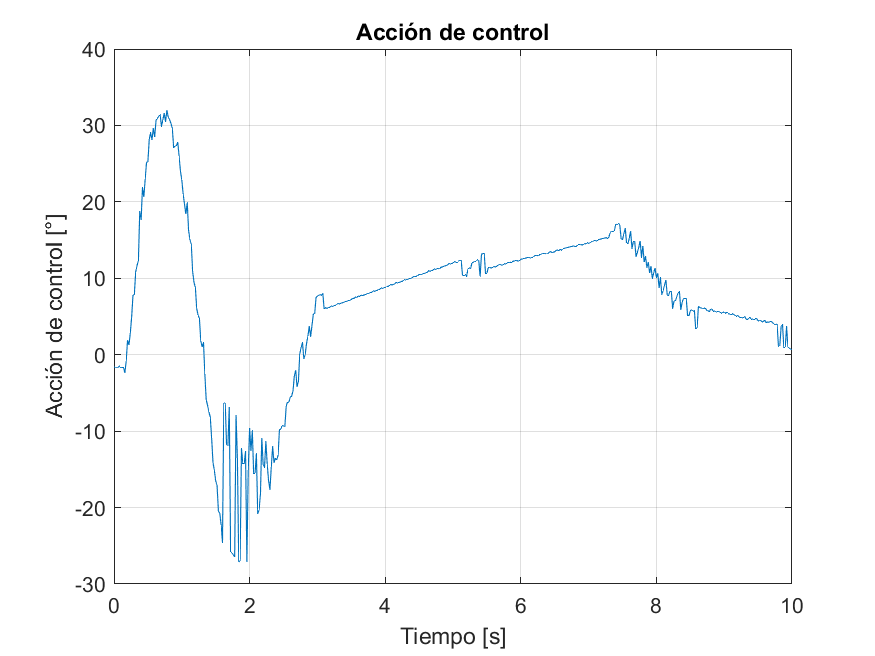
\includegraphics[width=\textwidth]{img/PI/PI-Acción de control(impulso).png}
    \caption{Acción de control ante impulso.}
    \label{fig:control_impulso_pi}
  \end{minipage}

  \vspace{0.4cm}

  \begin{minipage}{0.5\textwidth}
    \centering
    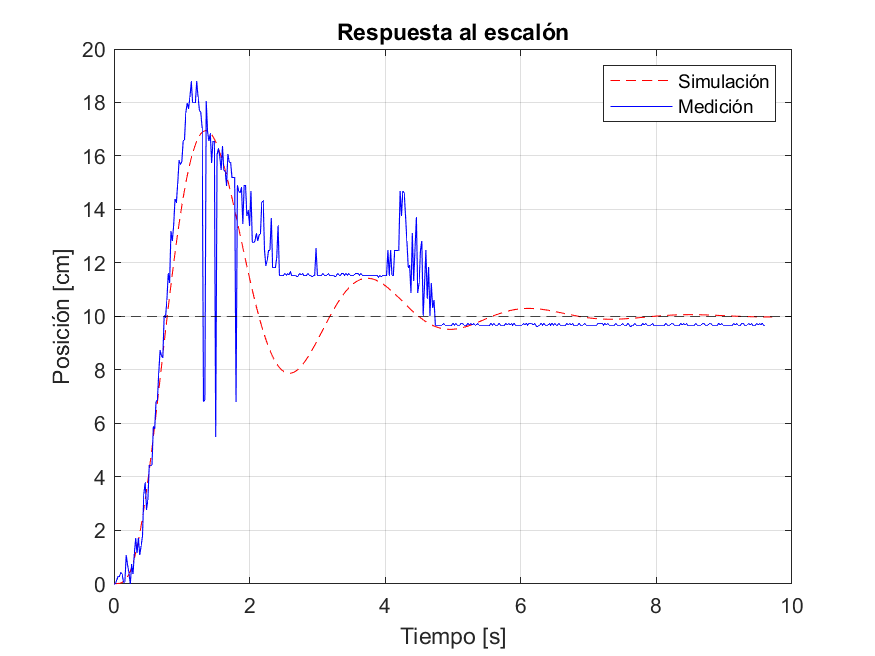
\includegraphics[width=\textwidth]{img/PI/PI-Respuesta al escalón.png}
    \caption{Respuesta al escalón de $T(s)$.}
    \label{fig:escalon_pi}
  \end{minipage}\hfill
  \begin{minipage}{0.5\textwidth}
    \centering
    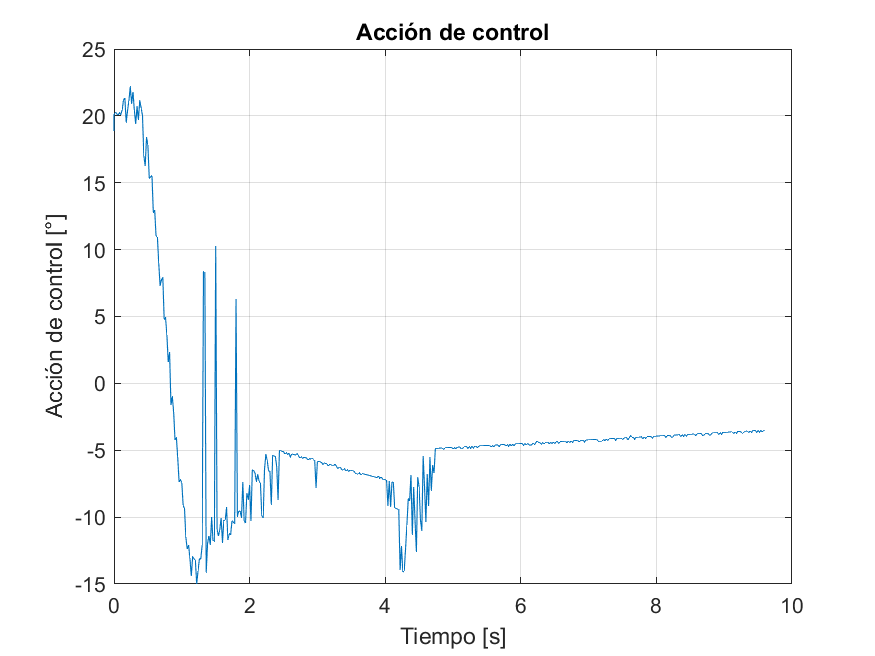
\includegraphics[width=\textwidth]{img/PI/PI-Acción de control(escalón).png}
    \caption{Acción de control ante escalón.}
    \label{fig:control_escalon_pi}
  \end{minipage}
\end{figure}

\subsection{Proporcional-Derivativo (PD)}

\label{sec:PD}
A la hora de implementar el control PD se encontraron varios problemas en la estimación de la derivada (\autoref{eq:derivada discreta}). 

\begin{figure}[H]
    \centering
    
\includegraphics[width=0.8\textwidth]{img/PD/PD-Derivada ruidosa.png}
    \caption{Error y su derivada.}
    \label{fig:derivada ruidosa}
\end{figure}

La \autoref{fig:derivada ruidosa} muestra el error medido por el sensor ultrasónico y su derivada calculada según la Ecuación \ref{eq:derivada discreta}. Puede notarse que esta última no es representativa de la derivada real del error, por lo que implementar un control PD con esta estimación resultaría problemático. El ruido intrínseco en la medición del sensor ultrasónico es la causa de la imprecisión en el cálculo de la derivada, por lo que para solucionar este problema sería necesario cambiar el sensor. Sin embargo, se encontró que, sin solucionar el problema de fondo, puede corregirse la estimación de la derivada para hacerla más representativa del comportamiento real del error.

En primer lugar, puede notarse en la \autoref{fig:derivada ruidosa} que la derivada oscila alrededor del 0. Este comportamiento se explica analizando la \autoref{eq:derivada discreta}. Nótese que el primer término de la misma $\left(\frac{2}{T_s}(e_k - e_{k-1})\right)$ podría resultar despreciable comparado con el segundo ($D_{k-1}$). Si esto ocurriera, en el instante $k$ se tendría que $D_k \approx - D_{k-1}$, con lo cual esta situación se propagaría al instante $k + 1$ y a los siguientes. Esto es, en efecto, lo que se observa en la \autoref{fig:derivada ruidosa}, en la que la derivada oscila entre $-2000$ y $2000$ aproximadamente. Esto explica por qué cuando el error se mantiene constante la derivada no es cero.

En segundo lugar, puede destacarse que valores tan elevados de la derivada resultan ilógicos. Si la derivada en el instante $k$ fuera realmente $2000\,\sfrac{\text{cm}}{\text{s}}$, el carrito se estaría moviendo a esa velocidad, o, lo que es equivalente, el carrito habría recorrido los \SI{40}{\cm} de la barra en tan solo un intervalo de muestreo. 

En base a estas dos observaciones se propone modificar el cálculo de la derivada de la siguiente forma: en primer lugar, ya que el sensor ultrasónico tiene una resolución mínima de $0,3\,$cm, si el cambio en el error es menor a esta cantidad, debe considerarse que no hay cambio real y forzar a que la derivada en ese instante sea nula. En segundo lugar, si el cambio en la medición del error es demasiado grande, debe considerarse que la medición es inválida y no se debe actualizar la derivada. De esta forma, se tienen dos umbrales, \texttt{UMBRAL\_INF} y \texttt{UMBRAL\_SUP}. Si $e_k - e_{k-1} < \text{\texttt{UMBRAL\_INF}}$, el cambio en el error es demasiado pequeño y se considera que $D_k = 0$. Si $e_k - e_{k-1} > \text{\texttt{UMBRAL\_SUP}}$ se considera que la medición es inválida y la derivada mantiene su valor.

\begin{figure}[H]
    \centering
    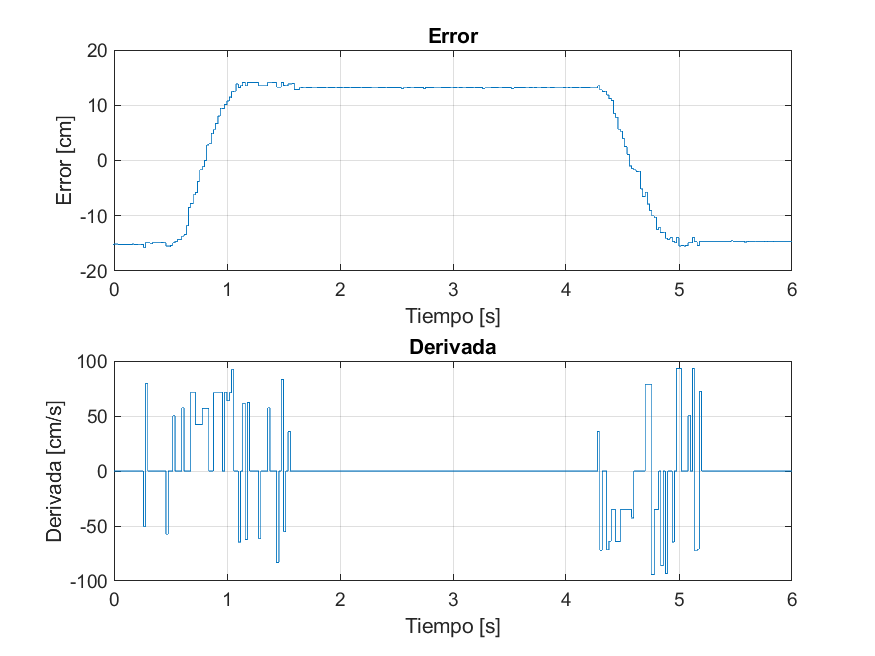
\includegraphics[width=0.8\textwidth]{img/PD/PD-derivada mejorada.png}
    \caption{Nueva estimación de la derivada}
    \label{fig:derivada mejorada}
\end{figure}

La Figura \ref{fig:derivada mejorada} muestra cómo queda la estimación de la derivada con estas limitaciones. Puede notarse que cuando el error es aproximadamente constante la derivada se mantiene en cero y que la misma es menos sensible al ruido de medición. Sin embargo, todavía presenta evidentes imperfecciones. Los umbrales elegidos fueron $\texttt{UMBRAL\_INF} = 0,3\,\text{cm}$ y $\texttt{UMBRAL\_SUP} = \SI{1}{\cm}$.

Similar al método seguido en las secciones anteriores, se eligieron $k_p = 2,5$ y $k_d = 0,1$ de forma tal de resolver el compromiso entre estabilidad y velocidad de respuesta de forma satisfactoria. En este caso, además, se buscó evitar la saturación de la acción de control. 

\begin{figure}[H]
    \centering
    
\includegraphics[width=0.8\textwidth]{img/PD/PD-Bode de L.png}
    \caption{Diagrama de Bode de $L(s)$.}
    \label{fig:PD-bode}
\end{figure}

\begin{figure}[H]
    \centering
    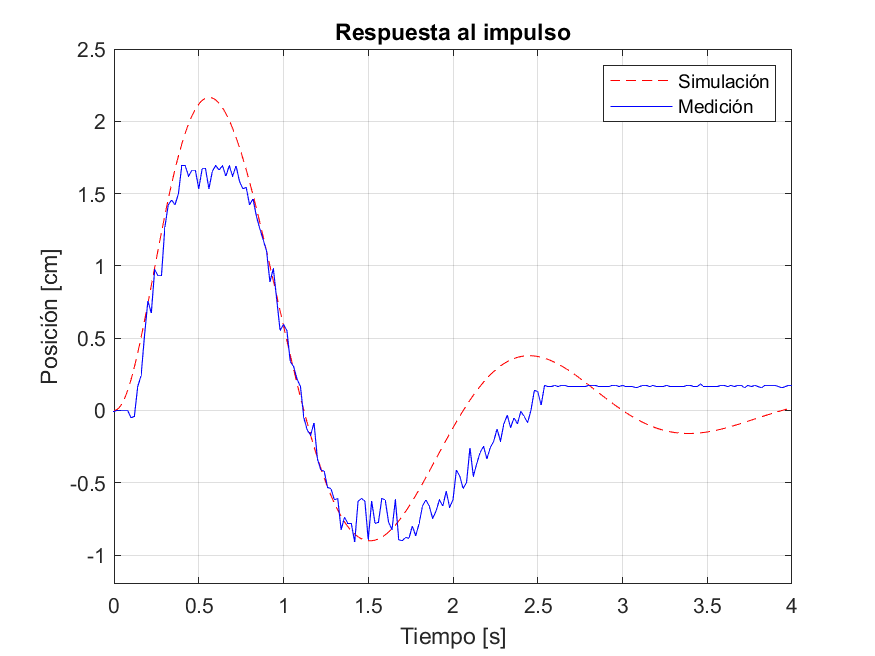
\includegraphics[width=0.8\textwidth]{img/PD/PD-Respuesta al impulso.png}
    \caption{Respuesta al impulso del control PD.}
    \label{fig:PD-respuesta al impulso}
    
\end{figure}

\begin{figure}[H]
    \centering
    
\includegraphics[width=0.8\textwidth]{img/PD/PD-Acción de control(escalón).png}
    \caption{Acción de control de la respuesta al impulso.}
    \label{fig:PD-acción de control impulso}
\end{figure}

\begin{figure}[H]
    \centering
    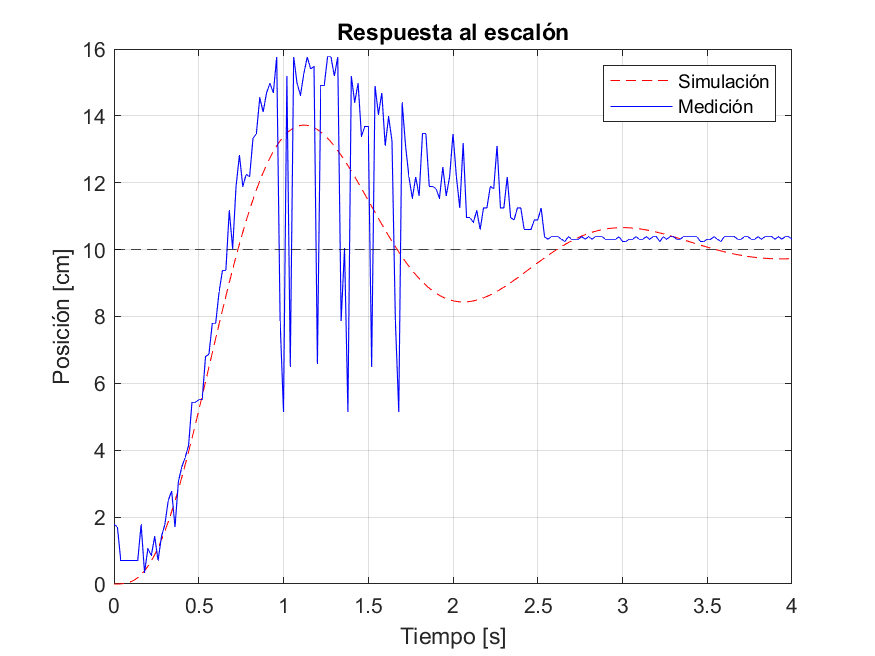
\includegraphics[width=0.8\textwidth]{img/PD/PD-Respuesta al escalón.png}
    \caption{Respuesta al escalón del control PD.}
    \label{fig:PD-respuesta al escalón}
\end{figure}

\begin{figure}[H]
    \centering
    
\includegraphics[width=0.8\textwidth]{img/PD/PD-Acción de control(escalón).png}
    \caption{Acción de control de la respuesta al escalón.}
    \label{fig:PD-acción de control escalón}
\end{figure}

Se observa tanto en la Figura \ref{fig:PD-respuesta al impulso} como en la \ref{fig:PD-respuesta al escalón} que la posición medida y la estimada son similares en algunos puntos y presentan evidentes diferencias en otros. Además, la posición logra estabilizarse en la referencia satisfactoriamente. Por otro lado, tanto en la Figura \ref{fig:PD-acción de control impulso} como en la \ref{fig:PD-acción de control escalón} se observa que se alcanzó el objetivo de no saturar la acción de control, cuyos límites se indican en línea negra rayada.

\section{Conclusiones}

En el desarrollo de este trabajo práctico se determinó la transferencia que modela la planta, así como un modelo en espacio de estados del sistema. Se determinaron también las limitaciones intrínsecas de las variables del modelo, lo que resultó fundamental a la hora de implementar los controladores.

Sobre el modelo hallado, se diseñaron tres controladores, uno proporcional, otro proporcional-integral y un último proporcional-derivativo. Todos los diseños se hicieron buscando resolver el compromiso entre velocidad de respuesta y estabilidad.

En el diseño del controlador PD se hicieron evidentes los problemas de ruido asociados a tal controlador. Utilizando el método explicado en la Sección \ref{sec:PD} el problema pudo ser resuelto solo de forma superficial. En futuros trabajos podría ser más útil implementar el control derivativo con otra estimación de la derivada. 

\section{Referencias}

[1] Morgan, Elijah J., \textit{HC-SR04 Ultrasonic Sensor}, 2014

[2] InvenSens Inc, \textit{MPU 6000 and 6050 Product Specification Revision 3.3.}, 2012.

[3] Handson Technology, \textit{MG996R Metal Gear Servo Motor.}

[4] Arduino, \textit{Arduino UNO R3 Product Reference Manual}, Rev. 3, 30/04/2024.

[5] Microchip Technology, \textit{ATmega328P Datasheet – 8-bit AVR Microcontroller}, Complete Datasheet.


\end{document}